\documentclass[../ESOF_notes.tex]{subfiles}
 
\begin{document} 

\paragraph{Biggest Web Security Risks:}
\begin{enumerate}
    \item Injection
    \item Broken Authentication
    \item Sensitive Data Exposure
    \item XML External Entities
    \item Broken Access Control
    \item Security Misconfiguration
    \item XSS
    \item Insecure Deserialization
    \item Componentes with Known Vulnerabilities
    \item Insufficient Logging \& Monitoring
\end{enumerate}

\subsection{SQL Injection}
Consider this query:
\begin{verbatim}
db.query("SELECT * FROM users WHERE email = '" + 
inputEmail + "' AND password = '" + inputPassword + "'");
\end{verbatim}
What happens when \textbf{inputPassword} has the following value? 
\code{' OR '1'='1}

\begin{verbatim}
SELECT * FROM users WHERE email = 'admin@fe.up.pt' 
AND password = '' OR '1'='1'
\end{verbatim}

\paragraph{Prevention:}
\begin{itemize}
    \item Never trust the user
    \item \textbf{Prepared statements}
    \item Stored procedures
    \item Hide error messages
    \begin{itemize}
        \item Blind injection is way harder to perform
    \end{itemize}
    \item \sout{Regular expressions}
    \item Web Application Firewall
\end{itemize}
\begin{center}
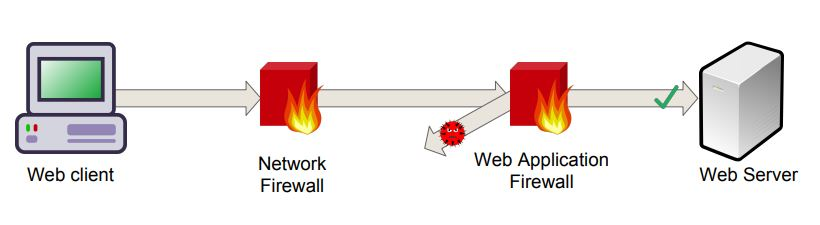
\includegraphics[scale=0.5]{WAF}
\end{center}


\subsection{Authentication} 

\paragraph{How to build a secure authentication system?}
\begin{center}
    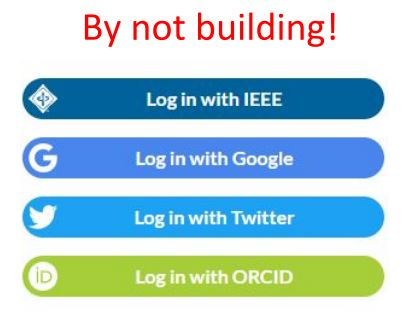
\includegraphics{AUTH}
\end{center}

\paragraph{Challanges:}
\begin{itemize}
    \item Password encryption
    \item Block "easy" password
    \item Limit failed attempts
    \item CSRF, Session forgery, ...
    \item Forgot my password
    \item Forgot my ID
    \item Multi-factor
    \item SSO
    \item Revoking sessions
    \item Reset all passwords after breaches
\end{itemize}

\paragraph{Sessions}\mbox{}\\

Typical workflow with sessions:
\begin{center}
    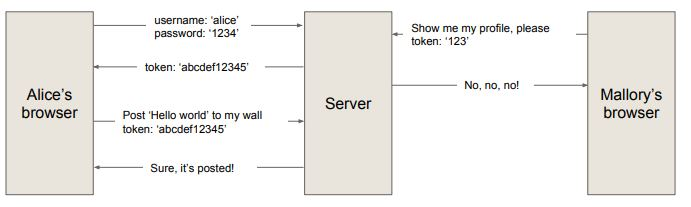
\includegraphics[scale=0.75]{session}
\end{center}

Session Tokens are usually stored in cookies.

\paragraph{Cookies}
\begin{center}
    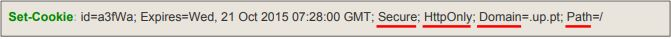
\includegraphics[scale=0.75]{cookie}
\end{center}
\begin{itemize}
    \item \textbf{Secure:} A secure cookie is only sent to the server with an encrypted request over the HTTPS protocol.
    \item \textbf{HttpOnly:} To prevent cross-site (XSS) attacks, HttpOnly cookies are inaccessible via Javascript.
    \item \textbf{Domain:} Domain specifies allowed hosts that will receive the cookie.
    \item \textbf{Path:} Path indicates a URL path that must exist in the requested URL in order to send the Cookie header.
\end{itemize}

\paragraph{Session Hijacking} \mbox{}\\

Sesion Hijacking is the exploitation of a valid computer session to gain unauthorized access to information or services in a computer system.

Main Methods:
\begin{itemize}
    \item Cross-site scripting
    \item Session fixation
    \item Non-secure communications
    \item Malware
\end{itemize}

\paragraph{Session Fixation} \mbox{}\\

Consider this scenario:
\begin{enumerate}
    \item Bruno knows that \code{https://unsafe.example.com} accepts session tokens from query strings.
    \item Bruno tells Chico to visit \code{https://unsafe.example.com?SID=123456789}.
    \item Chico clicks the URL and logs in with her credentials for \code{https://unsafe.example.com}.
\end{enumerate}

Chico is now using the session token \textbf{123456789}, which was provided by Bruno, so Bruno can use the same token to access Chico's account.
\newline

\quad \textbf{Prevention:}
\begin{itemize}
    \item Reject session identifiers from GET/POST variables.
    \item Regenerate the session token in every request.
    \begin{itemize}
        \item Not always possible
    \end{itemize}
    \item Regenerate the session ID when users log in.
\end{itemize}

\paragraph{JWT} \mbox{}\\

JSON web token is a standard that defines a compact and self-contained way for securely transmitting information between parties as a JSON object.

Use cases:
\begin{itemize}
    \item \textbf{Authorization:} Once the user is logged in, each subsequent request will include the JWT, allowing the user to access routes, services, and resources that are permitted with that token. It is also commonly used in SSO.
    \item \textbf{Information Exchange:} JWT is a good way of securely transmitting information between parties.
\end{itemize}

A JWT typically looks as: \code{<header>.<payload>.<signature>}

\begin{center}
    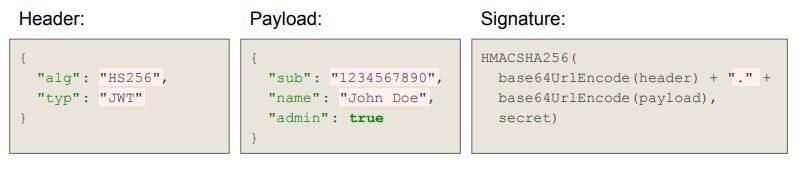
\includegraphics[scale=0.75]{JWT}
\end{center}

\begin{itemize}
    \item Header
    \begin{itemize}
        \item Base64Url encoded
    \end{itemize}
    \item Payload
    \begin{itemize}
        \item Base64Url encoded
    \end{itemize}
    \item Signature
    \begin{itemize}
        \item Signed using HMAC256
        \item Message: \code{Base64(header) + "." + Base64(payload)}
        \item Key: secret key
    \end{itemize}
\end{itemize}

\subsection{Cross-site scripting (XSS)}

\textbf{Cross-site scripting} is a type of attack where malicious code is injected in web pages trusted and viwed by other users.

\begin{center}
    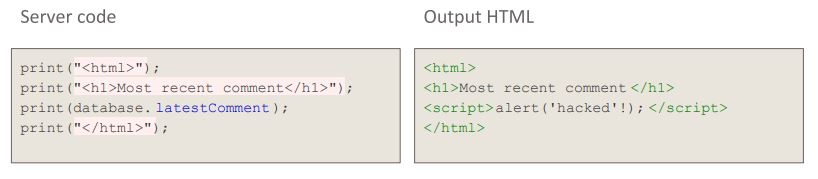
\includegraphics[scale=0.75]{XSS}
\end{center}

\paragraph{Prevention:} \mbox{}\\

Never trust user input...
\begin{itemize}
    \item Anywhere in your HTML document
    \item In CSS
    \item In a script
    \item ...
\end{itemize}

Make sure you always \textbf{encode} untrusted data.

\subsection{Sensitive Data Exposure}

\paragraph{Public-key cryptography:} \mbox{}\\

Public-key cryptography or asymmetric cryptography is an encryption scheme that uses two keys: a public key and a prive key. It is used to block \textbf{man-in-the-middle} attacks.

The private key is used to decrypt messages encrypted with the public key.

\paragraph{HTTPS:}\mbox{}\\

HTTPS uses public-key cryptography to establish secure connections.
The protocols works on top of TLS, which is an updated version of SLL.

\begin{center}
    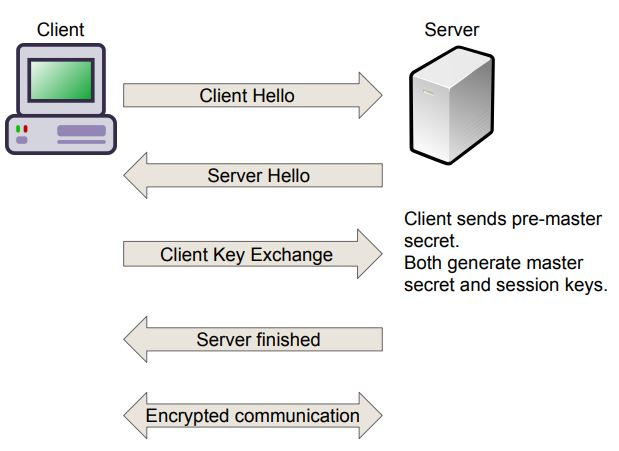
\includegraphics[scale=0.5]{HTTPS}
\end{center}

\paragraph{HSTS:}\mbox{}\\

\textbf{HTTP Strict Transport Security} is a web server directive that informs user agents and web browsers how to handle its connection.

\begin{center}
    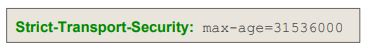
\includegraphics{STS}
\end{center}

HSTS headers tell the browser to:
\begin{enumerate}
    \item Always convert \code{http://} to \code{https://}.
    \item Block the connection if a secure connection cannot be established.
\end{enumerate}

\paragraph{Certificate Authorities:}\mbox{}\\

A \textbf{Certificate Authority (CA)} is an entity that issues digital certificates. Web browsers trust a predefined list of root CAs, that is shipped with the browser.

\paragraph{Handling passwords:}\mbox{}\\

A cryptographic hash function should have these properties:

\begin{itemize}
    \item Deterministic
    \item Fast to compute
    \item Non-invertible
    \item Changing a single byte in the message generates a totally different output
    \item Very hard to find collisions
\end{itemize}

If an intruder gains access to a database containing hashed passwords, there is no easy way of obtaining the original passwords.

However, he may take advantage of a \textbf{rainbow table}.

\textbf{Salts} help fighting rainbow tables and make password cracking more difficult.

\subsection{Security Misconfiguration}

\begin{itemize}
    \item Keeping default accounts
    \item Directory listing enabled
    \item Too much information in errors (such as stack traces)
    \item Out-of-date software
    \item Not disabling debug features
    \begin{itemize}
        \item If a debug feature is necessary then restrict access by user type and IP address.
    \end{itemize}
    \item ...
\end{itemize}

\subsection{CSRF}

Cross-Site Request Forgery attacks stem from the capability that a site has to issue a request to another site. Imagine a malicious website contains the following form:

\begin{center}
    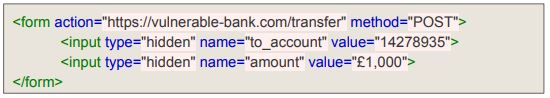
\includegraphics{CSRF}
\end{center}

The malicious website can use Javascript to submit that form for you. Since you have previously performed login in \code{https://vulnerable-bank.com},your money will be transferred.

\paragraph{Prevention:}
\begin{itemize}
    \item Anti-CSRF tokens \mbox{}\\
    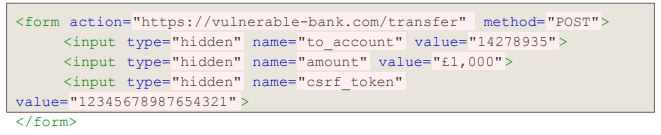
\includegraphics[scale=0.75]{Anti-CSRF}
    \item Same-site Cookies \mbox{}\\
    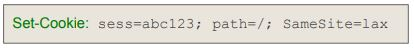
\includegraphics{SSC}
    \begin{itemize}
    \item Two modes: \code{strict} or \code{lax}
    \end{itemize}
\end{itemize}

\paragraph{Reverse Tabnabbing} \mbox{}\\

The following HTML is vulnerable to \textbf{Reverse Tabnabbing}:

\begin{center}
    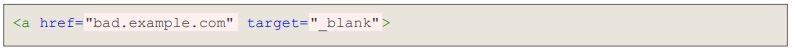
\includegraphics[scale=0.75]{RT}
\end{center}

Prevention is simple - add \code{rel="noopener"}:

\begin{center}
    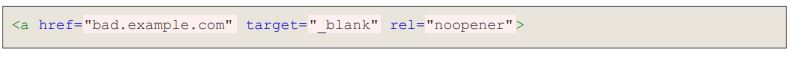
\includegraphics[scale=0.75]{NoRT}
\end{center}

\end{document}